%%%%%%%%%%%%%%%%%%%%%%%%%%%%%%%%%%%%%%%%%
% Beamer Presentation
% LaTeX Template
% Version 1.0 (10/11/12)
%
% This template has been downloaded from:
% http://www.LaTeXTemplates.com
%
% License:
% CC BY-NC-SA 3.0 (http://creativecommons.org/licenses/by-nc-sa/3.0/)
%
%%%%%%%%%%%%%%%%%%%%%%%%%%%%%%%%%%%%%%%%%

%----------------------------------------------------------------------------------------
%	PACKAGES AND THEMES
%----------------------------------------------------------------------------------------

\documentclass[10pt]{beamer}

\mode<presentation> {
	
	% The Beamer class comes with a number of default slide themes
	% which change the colors and layouts of slides. Below this is a list
	% of all the themes, uncomment each in turn to see what they look like.
	
	%\usetheme{default}
	%\usetheme{AnnArbor}
	%\usetheme{Antibes}
	%\usetheme{Bergen}
	%\usetheme{Berkeley}
	%\usetheme{Berlin}
	%\usetheme{Boadilla}
	%\usetheme{CambridgeUS}
	%\usetheme{Copenhagen}
	%\usetheme{Darmstadt}
	%\usetheme{Dresden}
	%\usetheme{Frankfurt}
	%\usetheme{Goettingen}
	%\usetheme{Hannover}
	%\usetheme{Ilmenau}
	%\usetheme{JuanLesPins}
	%\usetheme{Luebeck}
	\usetheme{Madrid}
	%\usetheme{Malmoe}
	%\usetheme{Marburg}
	%\usetheme{Montpellier}
	%\usetheme{PaloAlto}
	%\usetheme{Pittsburgh}
	%\usetheme{Rochester}
	%\usetheme{Singapore}
	%\usetheme{Szeged}
	%\usetheme{Warsaw}
	
	% As well as themes, the Beamer class has a number of color themes
	% for any slide theme. Uncomment each of these in turn to see how it
	% changes the colors of your current slide theme.
	
	%\usecolortheme{albatross}
	\usecolortheme{beaver}
	%\usecolortheme{beetle}
	%\usecolortheme{crane}
	%\usecolortheme{dolphin}
	%\usecolortheme{dove}
	%\usecolortheme{fly}
	%\usecolortheme{lily}
	%\usecolortheme{orchid}
	%\usecolortheme{rose}
	%\usecolortheme{seagull}
	%\usecolortheme{seahorse}
	%\usecolortheme{whale}
	%\usecolortheme{wolverine}
	
	\usefonttheme{serif}
	
	%\setbeamertemplate{footline} % To remove the footer line in all slides uncomment this line
	%\setbeamertemplate{footline}[page number] % To replace the footer line in all slides with a simple slide count uncomment this line
	
	%\setbeamertemplate{navigation symbols}{} % To remove the navigation symbols from the bottom of all slides uncomment this line
}
\usepackage{ragged2e}
\usepackage{lipsum}
\usepackage{amsmath}
\usepackage{gensymb}
\usepackage{textcomp}
\usepackage{braket}
\usepackage{lipsum}
\usepackage{bm}
\usepackage{graphicx, float} % Allows including images
\usepackage[centerlast]{subfigure}
\usepackage{wrapfig}
\usepackage{booktabs} % Allows the use of \toprule, \midrule and \bottomrule in tables
\usepackage{multicol}
\usepackage[font=scriptsize,labelfont=scriptsize]{caption}
\usepackage[spanish,es-tabla]{babel}
\usepackage[utf8]{inputenc}
\usepackage{csquotes}
\spanishdecimal{.}
\usepackage{gensymb}
\usepackage{textcomp}
\usepackage{amsmath}
\usepackage{nicefrac}

\usepackage{listings}
\usepackage{xcolor}

\usepackage{hyperref}
\hypersetup{
    colorlinks=true,
    linkcolor=black,
    filecolor=black,      
    urlcolor=blue,
    citecolor=black,
}
\urlstyle{same}

\definecolor{codegreen}{rgb}{0,0.6,0}
\definecolor{codegray}{rgb}{0.5,0.5,0.5}
\definecolor{codepurple}{rgb}{0.58,0,0.82}
\definecolor{backcolour}{rgb}{0.95,0.95,0.92}
\definecolor{codeblue}{RGB}{0, 180,201}
\definecolor{codered}{RGB}{238,25,0}



\lstdefinestyle{mystyle}{
	backgroundcolor=\color{backcolour},   
	commentstyle=\color{codeblue},
	keywordstyle=\color{codegreen},
	%numberstyle=\tiny\color{codegray},
	stringstyle=\color{codepurple},
	basicstyle=\ttfamily\footnotesize,
	breakatwhitespace=false,         
	breaklines=true,                 
	captionpos=b,                    
	keepspaces=true,                 
	%numbers=left,                    
	%numbersep=5pt,                  
	showspaces=false,                
	showstringspaces=false,
	showtabs=false,                  
	tabsize=2,
	moredelim=**[s][\color{codered}]{"""}{"""}
}

\lstset{emph={%  
		USE, KEYSPACE, WITH%
	},emphstyle={\color{codegreen}}%
}%

\lstset{literate = {á}{{\'a}}1 {é}{{\'e}}1 {í}{{\'i}}1 {Í}{{\'I}}1 {ó}{{\'o}}1 {ú}{{\'u}}1 {ñ}{{\~n}}1 {°}{{\textdegree}}1 {means-mu}{{$\mu$}}1 {std-sigma}{{$\sigma$}}1}

\lstset{language=Python, style=mystyle}

\newcommand\blfootnote[1]{%
  \begingroup
  \renewcommand\thefootnote{}\footnote{#1}%
  \addtocounter{footnote}{-1}%
  \endgroup
}

\setbeamertemplate{caption}[numbered]
%\captionsetup[figure]{font=scriptsize,labelfont=footnotesize}
%\captionsetup[subfigure]{font=scriptsize,labelfont=scriptsize}


%\makeatletter
%\newcommand\titlegraphicii[1]{\def\inserttitlegraphicii{#1}}
%\titlegraphicii{}
%\setbeamertemplate{title page}
%{
%	\vbox{}
%	{\usebeamercolor[fg]{titlegraphic}\inserttitlegraphic\hfill\inserttitlegraphicii\par}
%	\begin{centering}
%		\begin{beamercolorbox}[sep=8pt,center]{institute}
%			\usebeamerfont{institute}\insertinstitute
%		\end{beamercolorbox}
%		\begin{beamercolorbox}[sep=8pt,center]{title}
%			\usebeamerfont{title}\inserttitle\par%
%			\ifx\insertsubtitle\@empty%
%			\else%
%			\vskip0.25em%
%			{\usebeamerfont{subtitle}\usebeamercolor[fg]{subtitle}\insertsubtitle\par}%
%			\fi%     
%		\end{beamercolorbox}%
%		\vskip1em\par
%		\begin{beamercolorbox}[sep=8pt,center]{date}
%			\usebeamerfont{date}\insertdate
%		\end{beamercolorbox}%\vskip0.5em
%		\begin{beamercolorbox}[sep=8pt,center]{author}
%			\usebeamerfont{author}\insertauthor
%		\end{beamercolorbox}
%	\end{centering}
%	%\vfill
%}
%
%\titlegraphic{
\includegraphics[height=1.5cm,width=2cm]{unam.png}}
%\titlegraphicii{
\includegraphics[height=1.5cm,width=2cm]{unam.png}}

%----------------------------------------------------------------------------------------
%	TITLE PAGE
%----------------------------------------------------------------------------------------
\vspace*{3em}
\title[Ataques adversarios]{Ataques adversarios} % The short title appears at the bottom of every slide, the full title is only on the title page

\author[IIMAS, UNAM]{E. David Guzmán Ramírez} % Your name
\institute[] % Your institution as it will appear on the bottom of every slide, may be shorthand to save space
{	Licenciatura en Ciencia de Datos \\
	Introducción al Aprendizaje Profundo \\ \medskip M. en C. Berenice Montalvo Lezama \\ M. en C. Ricardo Montalvo Lezama
}
\date{{\tiny 23 de abril de 2021}} % Date, can be changed to a custom date

\vspace*{-5em}

\titlegraphic{
\includegraphics[width=1.8cm]{Images/unam.png}\hspace*{7.5cm}~%
	
\includegraphics[width=2.0cm]{Images/iimas.png} 
}

\begin{document}
	
	
\begin{frame}
	\titlepage % Print the title page as the first slide
\end{frame}

\begin{frame}
\frametitle{Contenidos}
\justify

\tableofcontents
\end{frame}

\section{Introducción}
\begin{frame}{Introducción}
\justify
\small
Las redes neuronales profundas son modelos poderosos que se han utilizado ampliamente para lograr un rendimiento cercano al nivel humano en una variedad de tareas. \medskip

Sin embargo, a pesar de su desempeño superior estudios recientes han encontrado que incluso los modelos del estado del arte son muy vulnerables a ataques adversarios.
\end{frame}

\begin{frame}{Introducción}
\justify
\small
Un ataque adversario es una muestra de datos de entrada que ha sido perturbada levemente con la intención de hacer fallar a un clasificador. 

\blfootnote{\vspace*{0.3cm} \href{https://arxiv.org/pdf/1412.6572.pdf}{Goodfellow et al., \emph{Explaining and harnessing adversarial examples}, 2016.}}

\begin{figure}
\centering
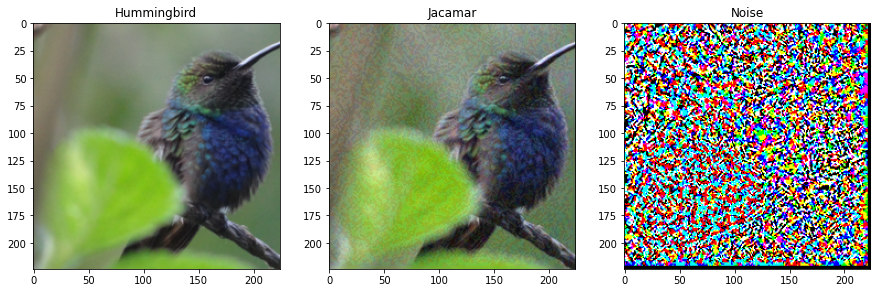
\includegraphics[width=0.85\linewidth]{Images/hummingbird_blackbox.png}
\caption{Ejemplo de ataque adversario. Imagen tomada de \href{https://arxiv.org/pdf/1412.6572.pdf}{\emph{Explaining and harnessing adversarial examples}.}}
\end{figure}

\end{frame}

\begin{frame}{Introducción}
\justify
\small

\blfootnote{\vspace*{0.3cm} \href{https://arxiv.org/pdf/1412.6572.pdf}{Su et al., \emph{One Pixel Attack for Fooling Deep Neural Networks}, 2019.}}

\begin{figure}
\centering
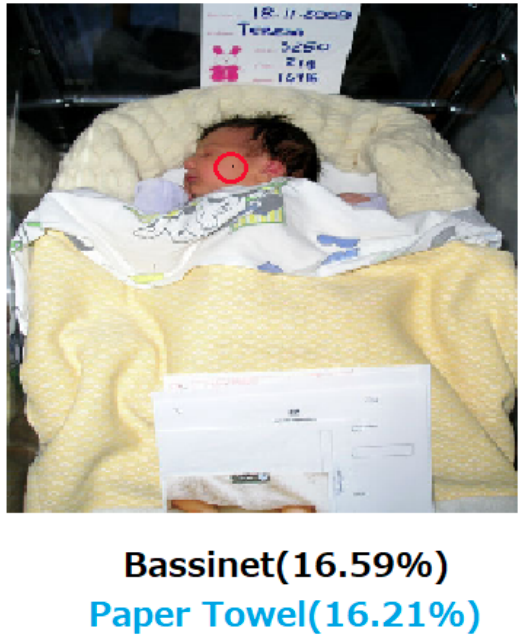
\includegraphics[width=0.3\linewidth]{Images/ejemplo3_anotado.png}
\caption{Ejemplo de ataque adversario en el que es posible engañar a la red cambiando únicamente un pixel. Imagen tomada de \href{https://arxiv.org/pdf/1710.08864.pdf}{\emph{One Pixel Attack for Fooling Deep Neural Networks}.}}
\end{figure}

\end{frame}

\begin{frame}{Introducción}
\justify
\small
Los escenarios de posibles ataques adversarios se pueden clasificar en diferentes maneras:

\begin{itemize}
\item \textbf{Ataque no dirigido:} el objetivo es hacer que el clasificador prediga una etiqueta incorrecta, la etiqueta incorrecta específica no importa.

\item \textbf{Ataque dirigido:} el objetivo es cambiar la predicción del clasificador a alguna clase objetivo específica.
\end{itemize}

\end{frame}

\begin{frame}{Introducción}
\justify
\small
En segundo lugar, los escenarios de ataque se pueden clasificar por la cantidad de conocimiento que el adversario tiene sobre el modelo:

\begin{itemize}
\item \textbf{Caja negra:} el atacante no sabe mucho sobre el modelo, pero puede sondear o consultar el modelo, es decir, darle algunas entradas y observar salidas.

\item \textbf{Caja blanca:} el atacante tiene pleno conocimiento del modelo, como la arquitectura del modelo y los valores de todos los parámetros y pesos entrenables.
\end{itemize}

\end{frame}


\section{Motivación}
\begin{frame}{Motivación}
\justify
\small
Los ataques adversarios plantean problemas de seguridad porque podrían usarse para realizar un ataque a los sistemas de aprendizaje profundo, incluso si el atacante no tiene acceso al modelo subyacente. \medskip

Con la introducción de modelos de aprendizaje profundo en cada vez más distintos aspectos de nuestra vida, los problemas que estos ataques adversarios pueden ocasionar son preocupantes.

\end{frame}

\begin{frame}{Motivación}
\justify
\small

\begin{figure}
\centering
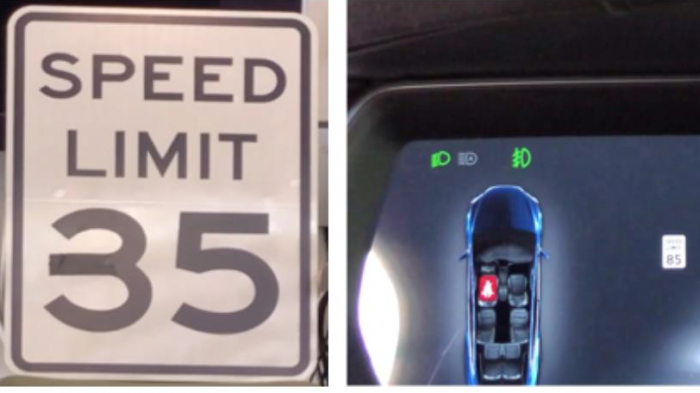
\includegraphics[width=0.65\linewidth]{Images/ejemplo2_anotado.png}
\caption{Ataque adversario al sistema de navegación autónomo de un Tesla, en el que confunde un señalamiento de velocidad de 35 millas/hora por 85 millas/hora. Figura tomada de \href{https://www.technologyreview.com/2020/02/19/868188/hackers-can-trick-a-tesla-into-accelerating-by-50-miles-per-hour/}{MIT Technology Review: Trick a Tesla into accelerating by 50 miles per hour.}}
\end{figure}

\end{frame}

\section{Descripción del problema}
\begin{frame}{Descripción del problema}
\justify
\small
Para acelerar la investigación sobre ataques de adversarios, Google Brain organizó la  \emph{Competencia de Ataques y Defensas Adversarios} en la edición de 2017 de NIPS, la cual está disponible en \href{https://www.kaggle.com/c/nips-2017-non-targeted-adversarial-attack/overview}{Kaggle}, la competencia a su vez constaba de tres subcompeticiones:

\begin{itemize}
\item Ataques adversarios no dirigido.
\item Ataques adversarios dirigido.
\item Defensas contra ataques adversarios.
\end{itemize}

Por el momento me concentraré en los ataques adversarios no dirigidos, la cual trata de un ataque de caja negra no dirigido, es decir, dada una imagen de entrada generar una imagen adversaria que engañe a un clasificador desconocido.

\end{frame}

\section{Análisis exploratorio}
\begin{frame}{Análisis exploratorio}
\justify	
\small

El dataset para esta competencia debía cumplir con 3 aspectos:

\begin{enumerate}
\item Conjunto de datos suficientemente grande y problema no trivial.
\item Problema bien conocido, por lo que las personas potencialmente pueden reutilizar los clasificadores existentes.
\item Muestras de datos que nunca se usaron antes.
\end{enumerate}

El conjunto de ImageNet cumple con los primeros dos requisitos, posteriormente se etiquetaron 1000 nuevas imágenes compatibles con ImageNet las cuales servían como el conjunto de datos de desarrollo para la competencia y para cumplir el tercer requisito.

\end{frame}

\section{Propuesta de solución}
\begin{frame}{Propuesta de solución}
\justify	
\small

Hay una variedad de arquitecturas preentrenadas en \href{https://pytorch.org/vision/stable/models.html}{PyTorch} con el conjunto de datos de ImageNet que sirven a la perfección para esta tarea. La idea es tratar de implementar varias técnicas de ataques adversarios\footnote{\vspace*{0.3cm} \href{https://reader.elsevier.com/reader/sd/pii/S209580991930503X?token=D051F74ED28FC5C7871D901893E9DAA76D35478F8C374211EC76DA66B1D71487CCB669164F543A5F3A04AE89239AC6C9&originRegion=us-east-1&originCreation=20210425231353}{Kui Ren et al., \emph{Adversarial Attacks and Defenses in Deep Learning}, 2020.}} sobre estas arquitecturas, como 

\begin{itemize}
\item \textbf{Métodos de gradiente:} la idea es $\bm{x}_{\text{adversario}} = \bm{x} + f(\nabla_{x}J(\bm{\theta}, \bm{x}, y))$.

\item \textbf{Métodos de distribución:} realiza la optimización sobre las posibles distribuciones adversarias.

\item \textbf{Basados en GANs: } un generador es entrenado para aprender la distribución adversaria maximizando la función de pérdida $J(\bm{\theta}, \bm{x}, y)$.
\end{itemize}


\end{frame}

\begin{frame}{Propuesta de solución}
\justify	
\small
Por ejemplo, usando un PGD\footnote{\vspace*{0.3cm} \href{https://arxiv.org/pdf/1706.06083.pdf}{A. Madry et al., \emph{Towards Deep Learning Models Resistant to Adversarial
Attacks}, 2019.}} en un clasificador entrenado en CIFAR10

\begin{figure}
\centering
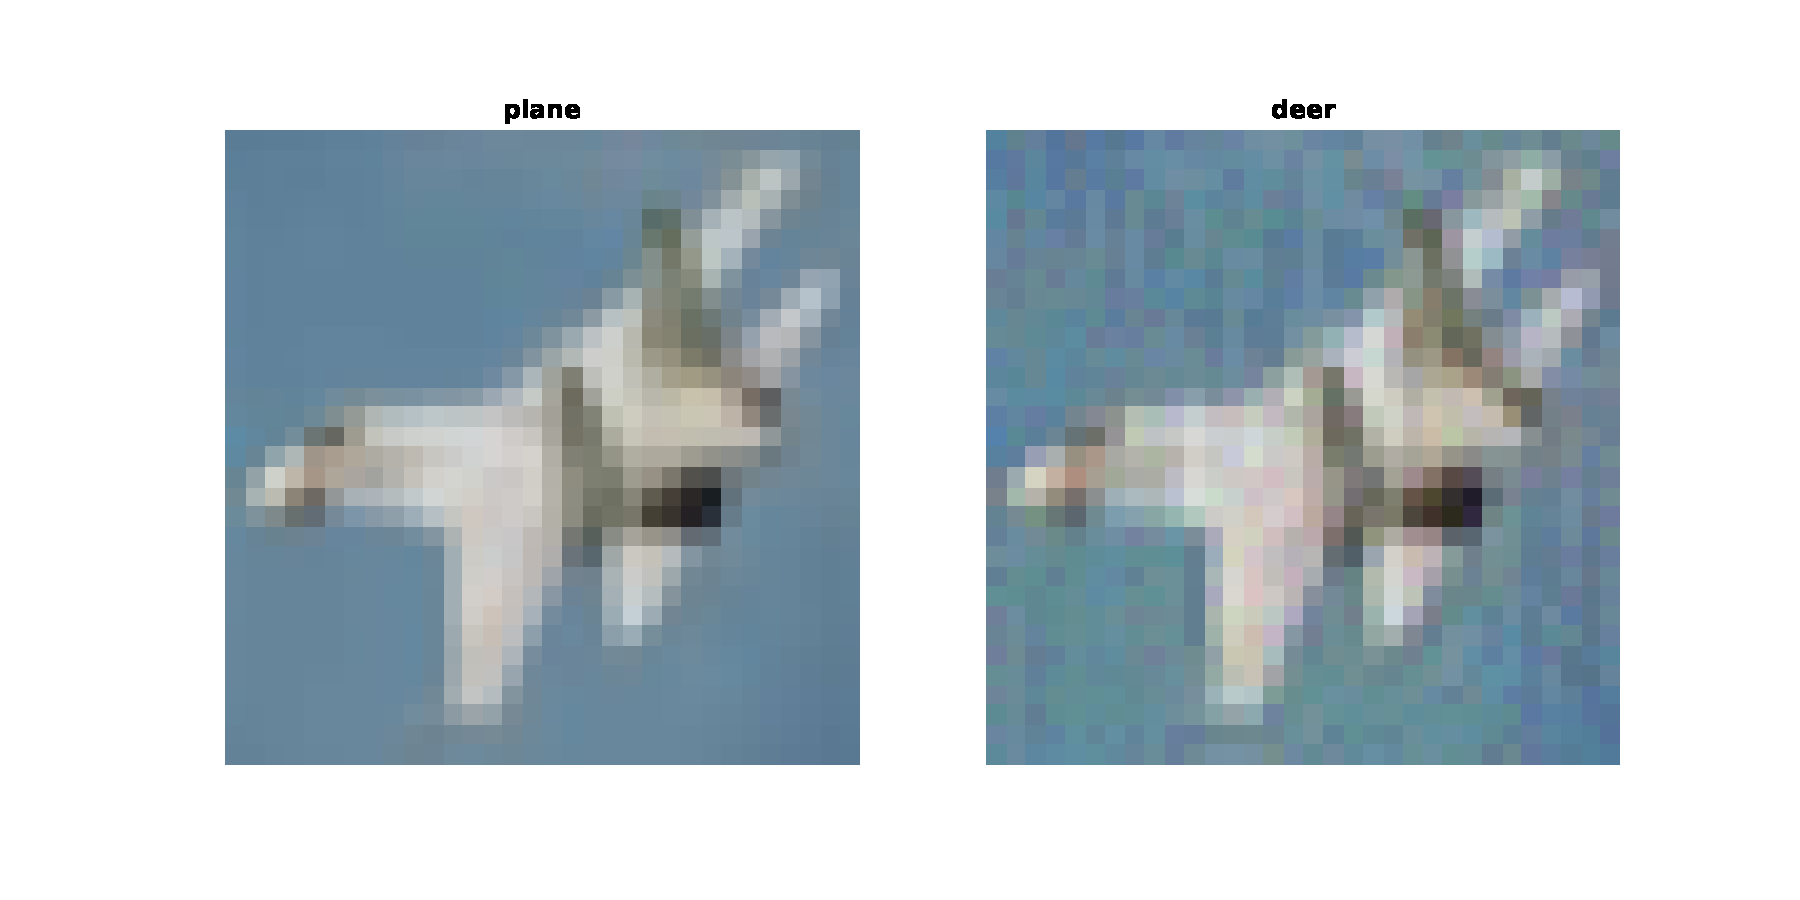
\includegraphics[width=0.65\linewidth]{Images/plane.pdf}
\caption{Ejemplo de un ataque adversario usando el dataset de CIFAR10.}
\end{figure}

\end{frame}

\section{Trabajo por hacer}
\begin{frame}{Trabajo por hacer}
\justify	
\small

\begin{itemize}
\item Usar los modelos preentrenados de \href{https://pytorch.org/vision/stable/models.html}{PyTorch} para hacer ataques en un dataset de prueba.

\item Una propuesta para defensa de ataques adversarios es entrenar el modelo con una mezcla de imágenes limpias y adversarias \footnote{\href{https://arxiv.org/pdf/1412.6572.pdf}{Goodfellow et al., \emph{\vspace*{0.3cm} Explaining and harnessing adversarial examples}, 2016.}}, por lo que con los ataques generados es posible construir un modelo más robusto resistente a los ataques.  
\end{itemize}

\end{frame}

%\section{Bibliografía}
%\begin{frame}{Bibliografía}
%\justify
%
%\footnotesize{
%
%\begin{thebibliography}{00}
%\bibitem{goodfellow-2014}
%\emph{\href{https://arxiv.org/pdf/1412.6572.pdf}{Link Prediction Using Supervised Learning}}, Mohammad Hasan, Vineet Chaoji, Saeed Salem, Mohammed Javeed Zaki, 2006.
%
%\bibitem{dblp-dataset}
%\emph{\href{https://dblp.org/faq/1474679.html}{Digital Bibliography \& Library Project (DBLP) dataset}},  Schloss Dagstuhl.
%\end{thebibliography}
%}
%
%\end{frame}

\end{document}
